%\info{Ben, Andrzej, Jesse, Gregory, Grigorios, Frederic}

The purpose of this section is to make some numerical estimates of the $\alpha_s$ extraction at the LHC.  Many simplifying assumptions are made, with the goal of motivating a more complete effort within the context of ATLAS and CMS in collaboration with theorists.   First, Sec~\ref{sec:templates} illustrates how $\alpha_s$ and the gluon fraction can be simultaneously extracted from the distribution of various angularities.  Next, Sec.~\ref{sec:resolution} estimates the needed experimental precision required to make a useful measurement of $\alpha_s$.   While both the theory and experimental precision will continue to improve over the next years, the community has already demonstrated that the work can begin with the first round of results~\cite{Aaboud:2017qwh,CMS-PAS-SMP-16-010,Frye:2016aiz,Frye:2016okc,Marzani:2017mva,Marzani:2017kqd}.

\subsection{Extraction of Theory Templates}
\label{sec:templates}

A complete extraction of $\alpha_s$ will require matching resummed results to high fixed order and also estimating non-perturbative effects.  The two sets of predictions for dijets thus far have matched to LO~\cite{Frye:2016aiz,Frye:2016okc} and NLO~\cite{Marzani:2017mva,Marzani:2017kqd} and have used PS MC to study non-perturbative corrections~\cite{Marzani:2017mva,Marzani:2017kqd}.  Performing high-order fixed order matching is computationally expensive; while this will be required eventually, we focus here on a conceptual demonstration.  Therefore, we focus on the resummation regime ($\ecf{2}{\alpha}\gtrsim \left. \ecf{2}{\alpha} \right |_{\text{NP}}$ - see Eq.~\ref{eq:np} and $\ecf{2}{\alpha}\lesssim z_\text{cut}R^\alpha$), where next-to-leading logarithmic calculations exist in analytic formulae that can be varied on-the-fly~\cite{Marzani:2017mva,Marzani:2017kqd}.  Regions of phase space that are highly sensitive to non-perturbative or fixed-order effects are removed.  Pseudo-data are then generated from the binned analytic probability distribution $t(\alpha_s,f_g)$.  These distributions are a superposition of the quark and gluon distributions and depend only on $\alpha_s$.  The pseudo-dataset has $n$ events and its binned representation is denoted by  $h(\alpha_s,f_g,n)$.  For a given pseudo-dataset, the fitted values of $\alpha_s$ and $f_g$ are determined from a $\chi^2$-like fit:

\begin{align}
\label{eq:chi2fit}
\alpha_s,f_g=\text{argmin} \sum_i (h_i(\alpha_s,f_g,n)-t_i(\alpha_s,f_g))^2/\sigma(h_i(\alpha_s,f_g,n)^2),
\end{align}

\noindent where $t_i, h_i$ are the bin content of histograms $t$ and $h$ while $\sigma(h_i)$ is the statistical uncertainty in bin $i$ of histogram $h$.  In practice, there would also be systematic uncertainties (see Sec.~\ref{sec:resolution}), but the purpose of this section is simplify illustrate the sensitivity to $\alpha_s$ and $f_g$ for a given number of events.  Figure~\ref{fig:templates} shows the quark and gluon templates for $\alpha=1$ and $2$ and $\beta=0$ and $1$.  The $\alpha=2$ fit is demonstrated in Fig.~\ref{fig:alpha2fit}.  The left plot of Fig.~\ref{fig:alpha2fit} shows the $\chi^2$ from Eq.~\ref{eq:chi2fit} for two samples, one with 20\% gluons and one with 80\% gluons.  The true value of $\alpha_s=0.1$, and as expected, the $\chi^2$ probability is high\footnote{It is not necessarily peaked at this value because this is the result of one pseudo-experiment.  Averaging over many pseudo-experiments results in peaks at $f_g=0.2$ and $0.8$.} for $f_g=0.2$ and $f_g=0.8$.  The banana shapes of the curves are a consequence of the degeneracy due to Casimir scaling discussed in Sec.~\ref{sec:casimir}.  From one sample alone, there is essentially no ability to distinguish between a larger $\alpha_s$ and a smaller $f_g$; the only constraint comes from the fact $0\leq f_g\leq 1$ which results in a crude bound on $\alpha_s$.  This is shown in the right plot of Fig.~\ref{eq:chi2fit} where the distribution is marginalized over $f_g$ and normalized to unity.  One can view this as the posterior probability of the fitted $\alpha_s$: the peak is the fitted value of $\alpha_s$ and the width is the uncertainty.  When $f_g$ is known, the uncertainty in $\alpha_s$ is significantly reduced; this is illustrated with pure quark and gluon samples.  Due to the larger color factor, the measurement with pure gluon jets is more sensitive to $\alpha_s$ than the fit using pure quark jets.  Using both the $f_g=0.2$ and $f_g=0.8$ samples to fit for $\alpha_s$, one can extract a $\sim 30\%$ measurement of $\alpha_s$.  However, there is no clear peak at the correct value of $\alpha_s$ due to the Casimir degeneracy.  

\begin{figure}[h!]
\begin{center}
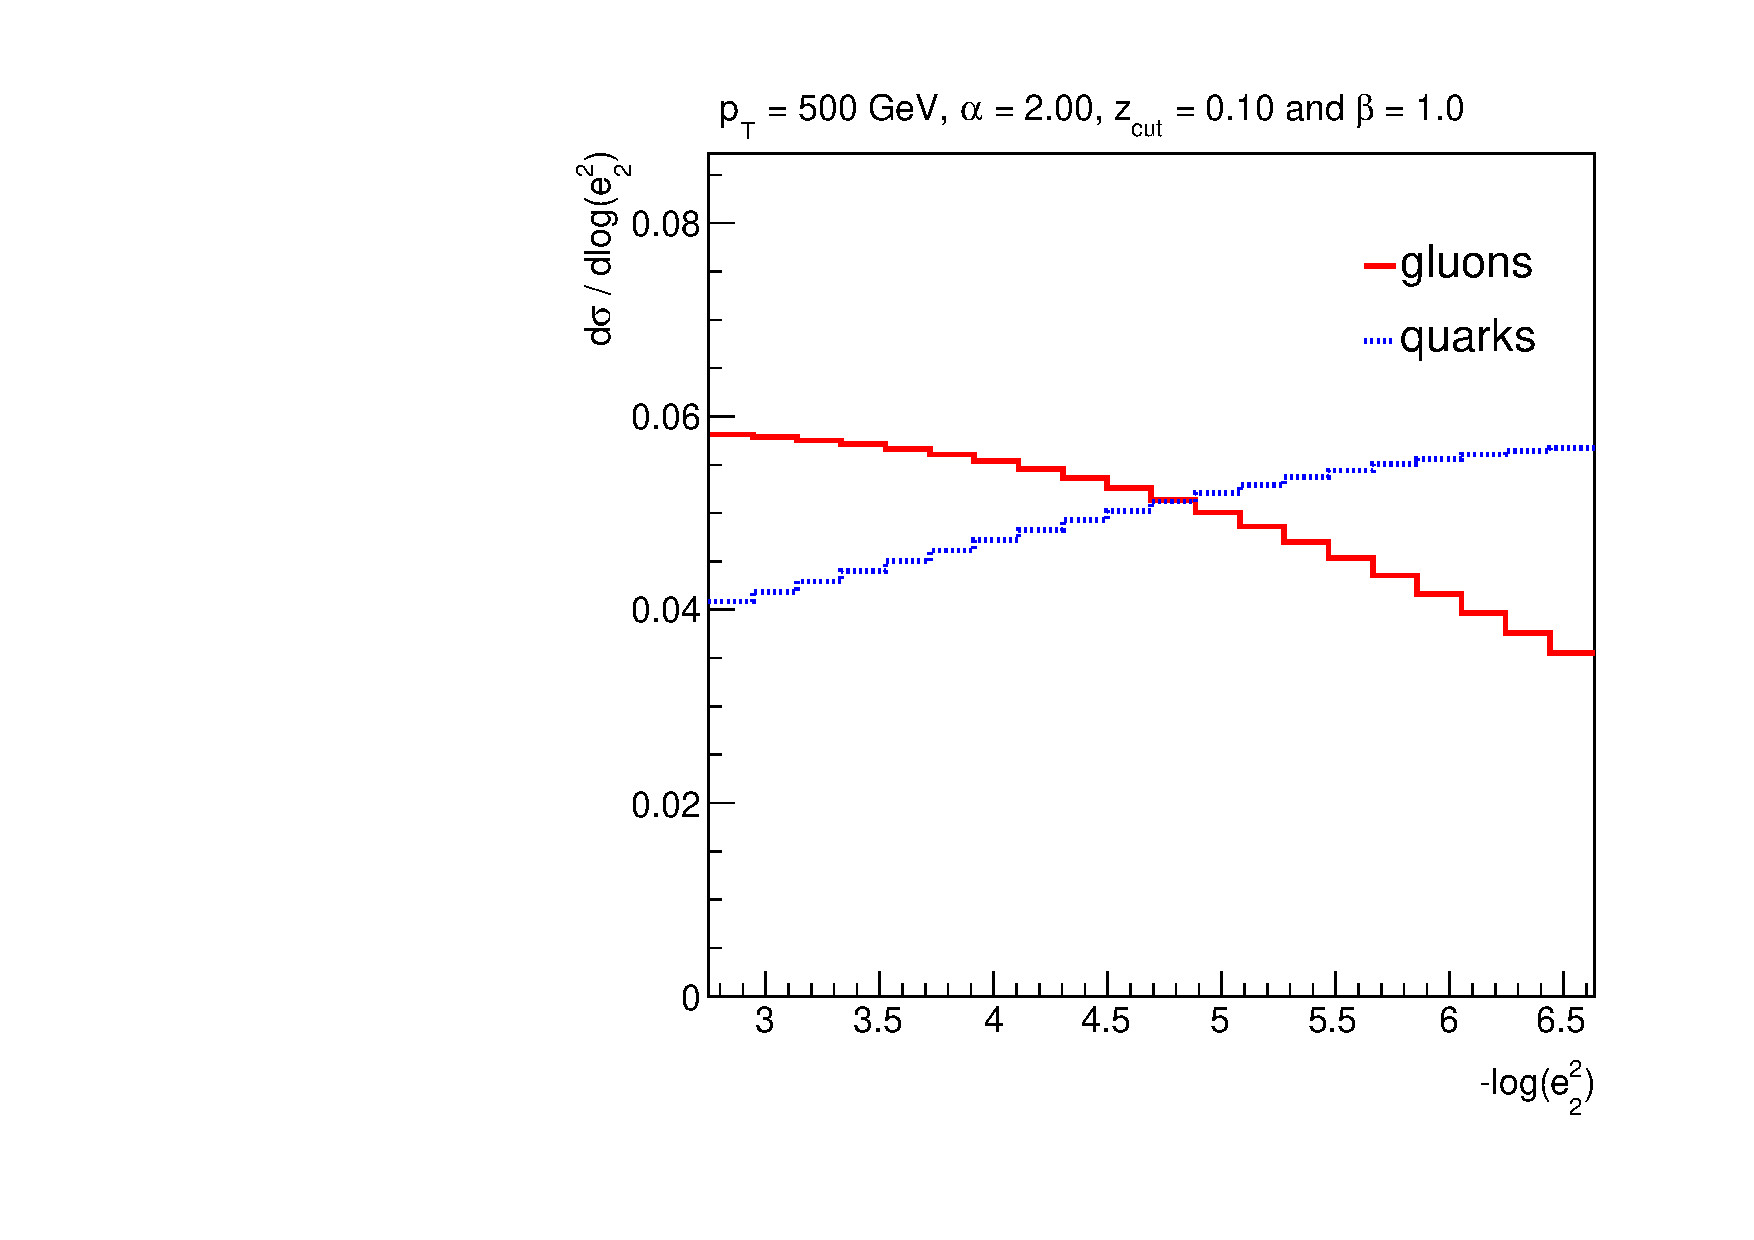
\includegraphics[width = 0.49\columnwidth]{figures/PDFs_alpha_20zcut1_beta_1023451324.pdf}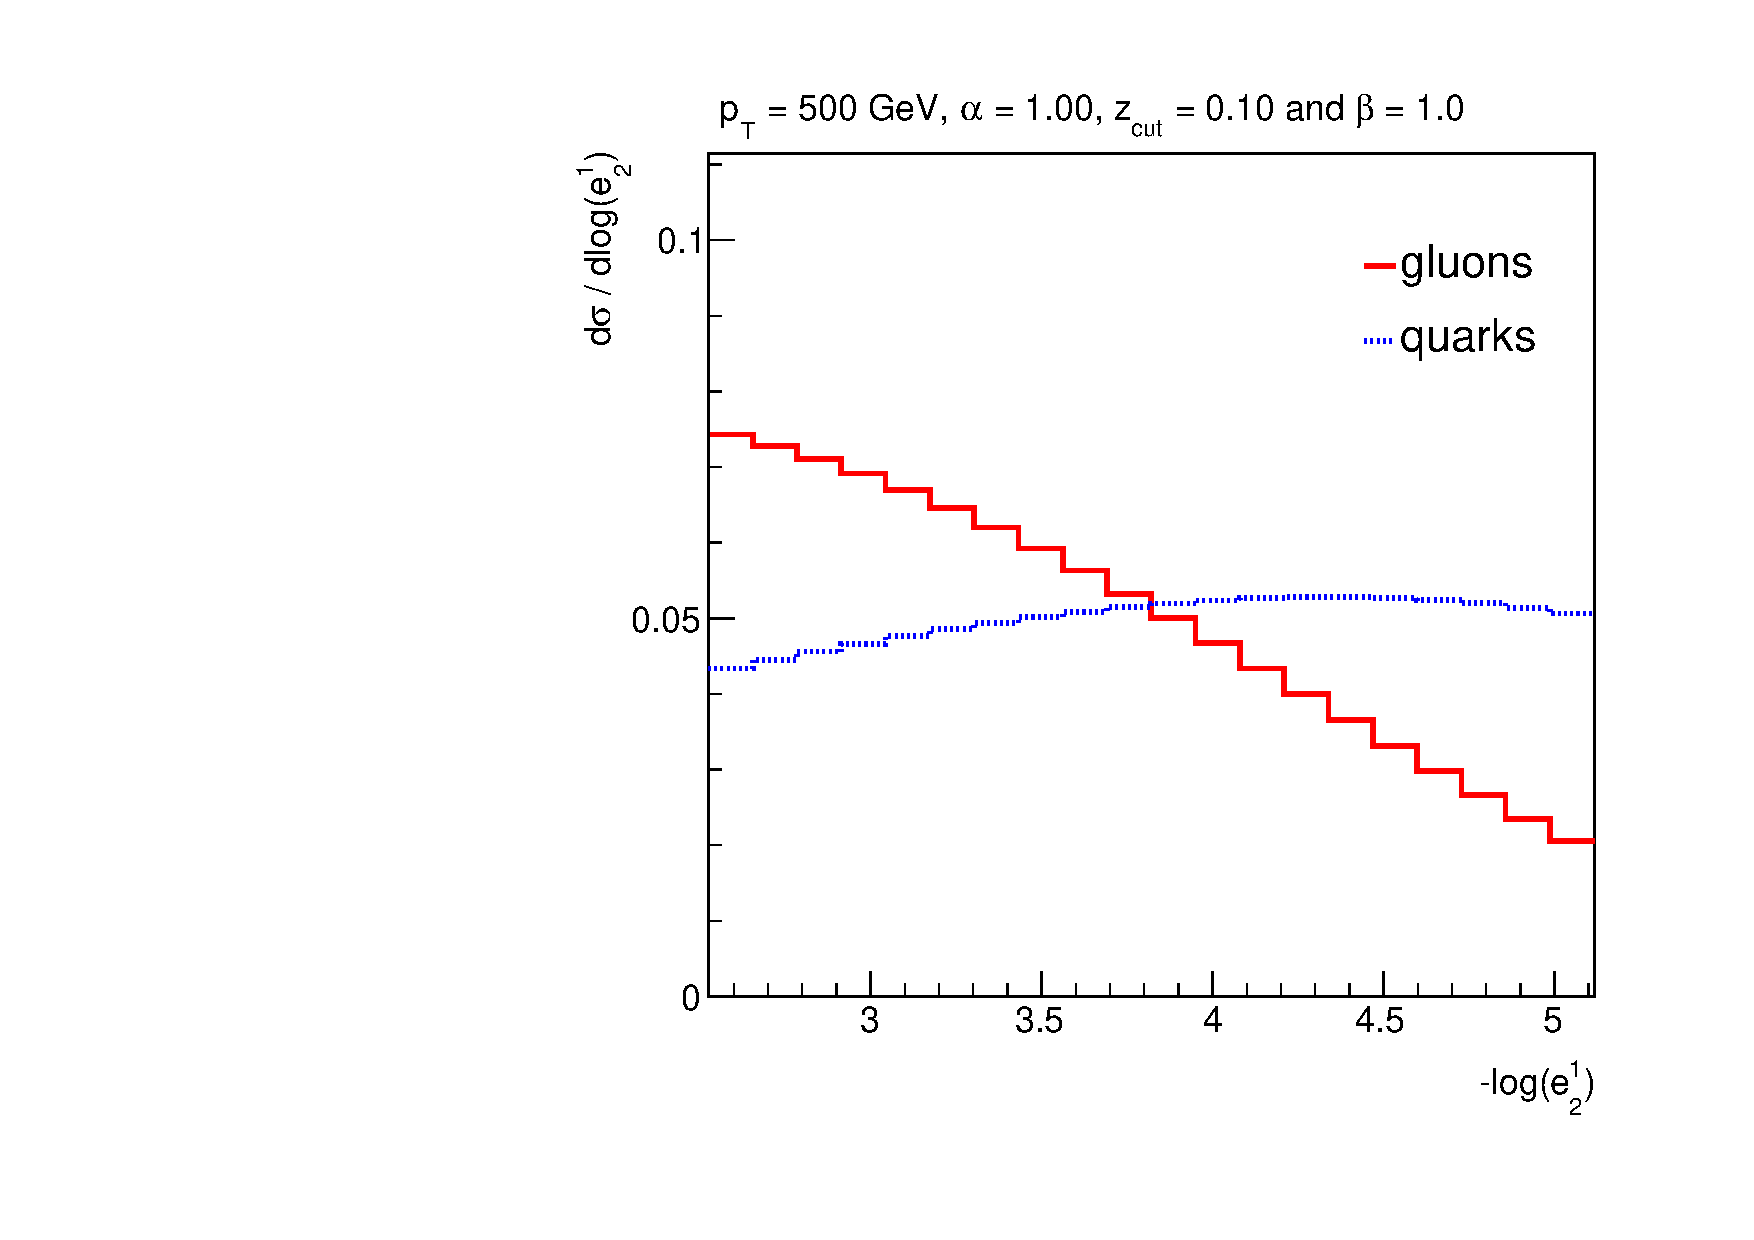
\includegraphics[width = 0.49\columnwidth]{figures/PDFs_alpha_10zcut1_beta_1023451324.pdf}\\
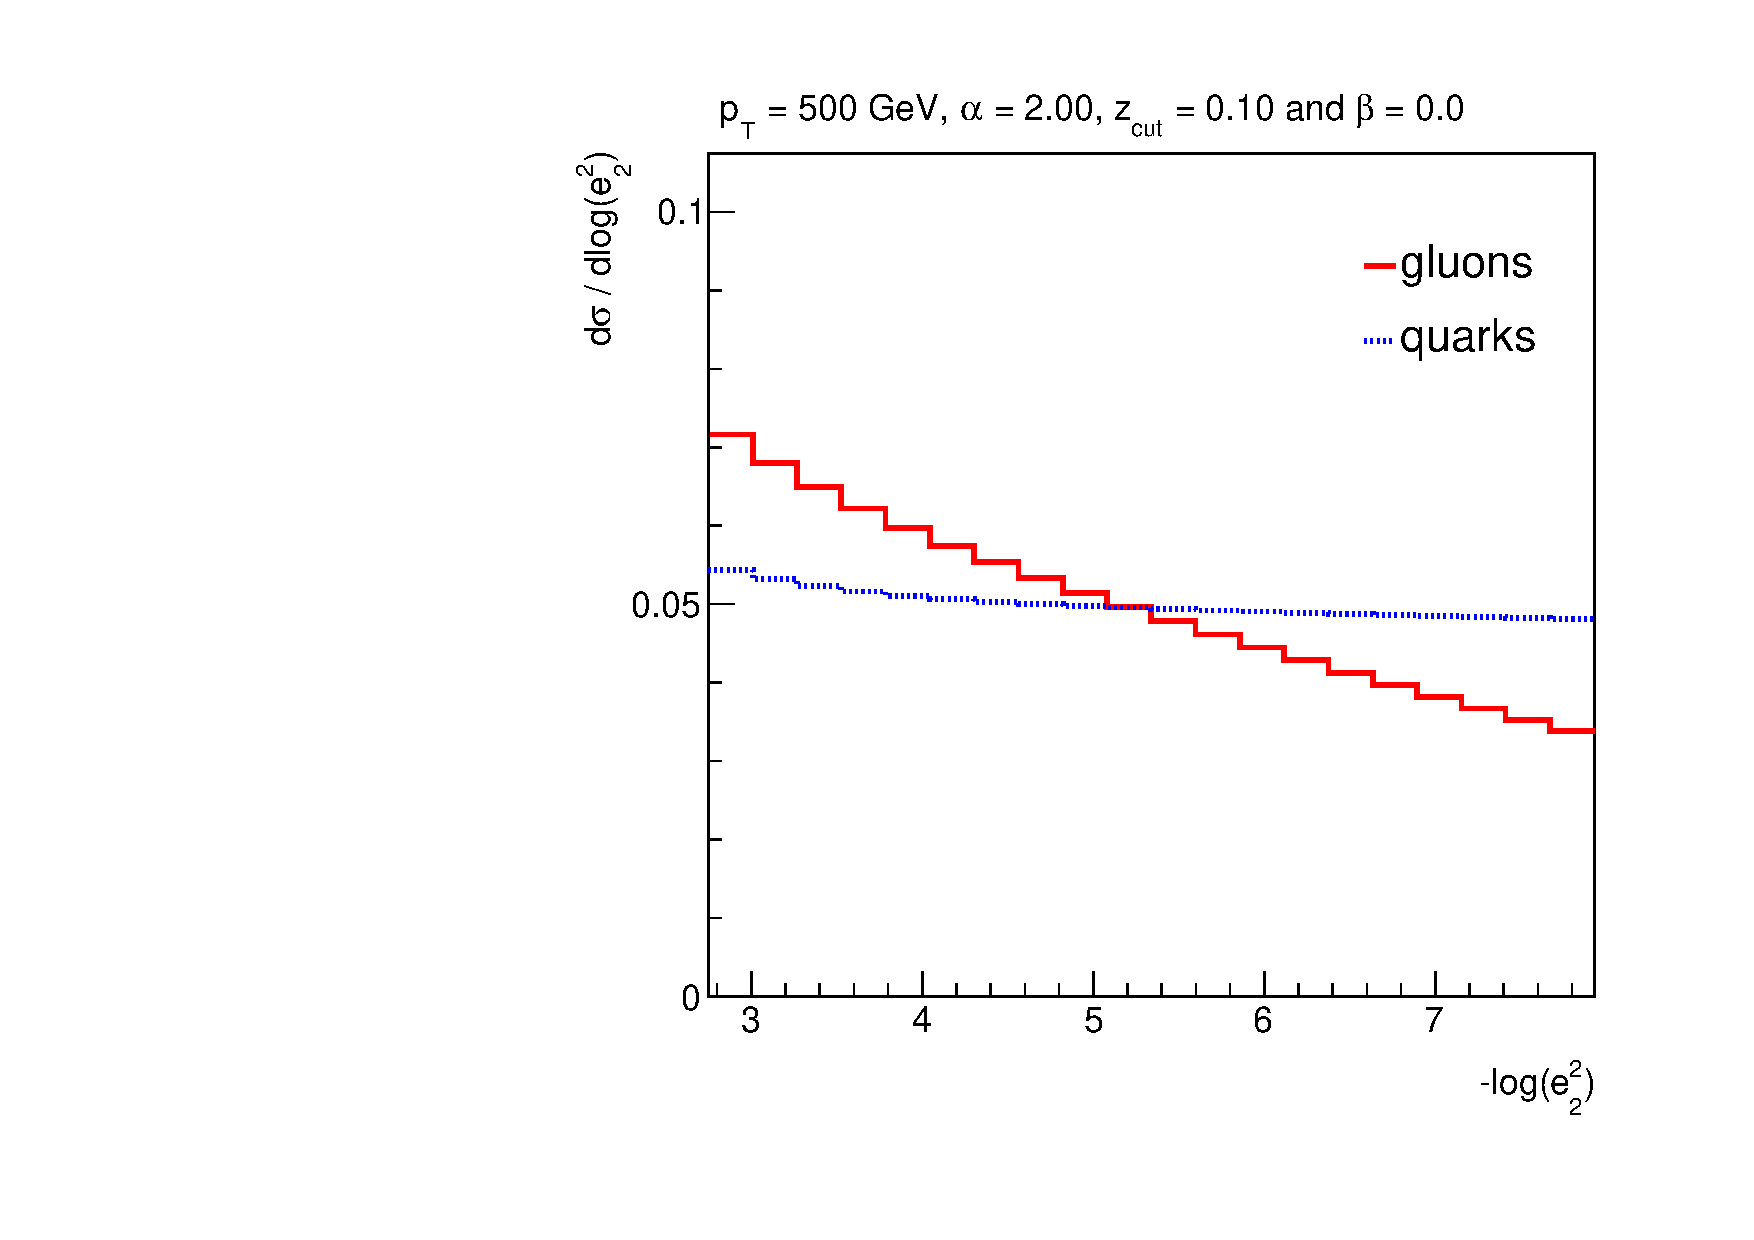
\includegraphics[width = 0.49\columnwidth]{figures/PDFs_alpha_20zcut1_beta_023451324.pdf}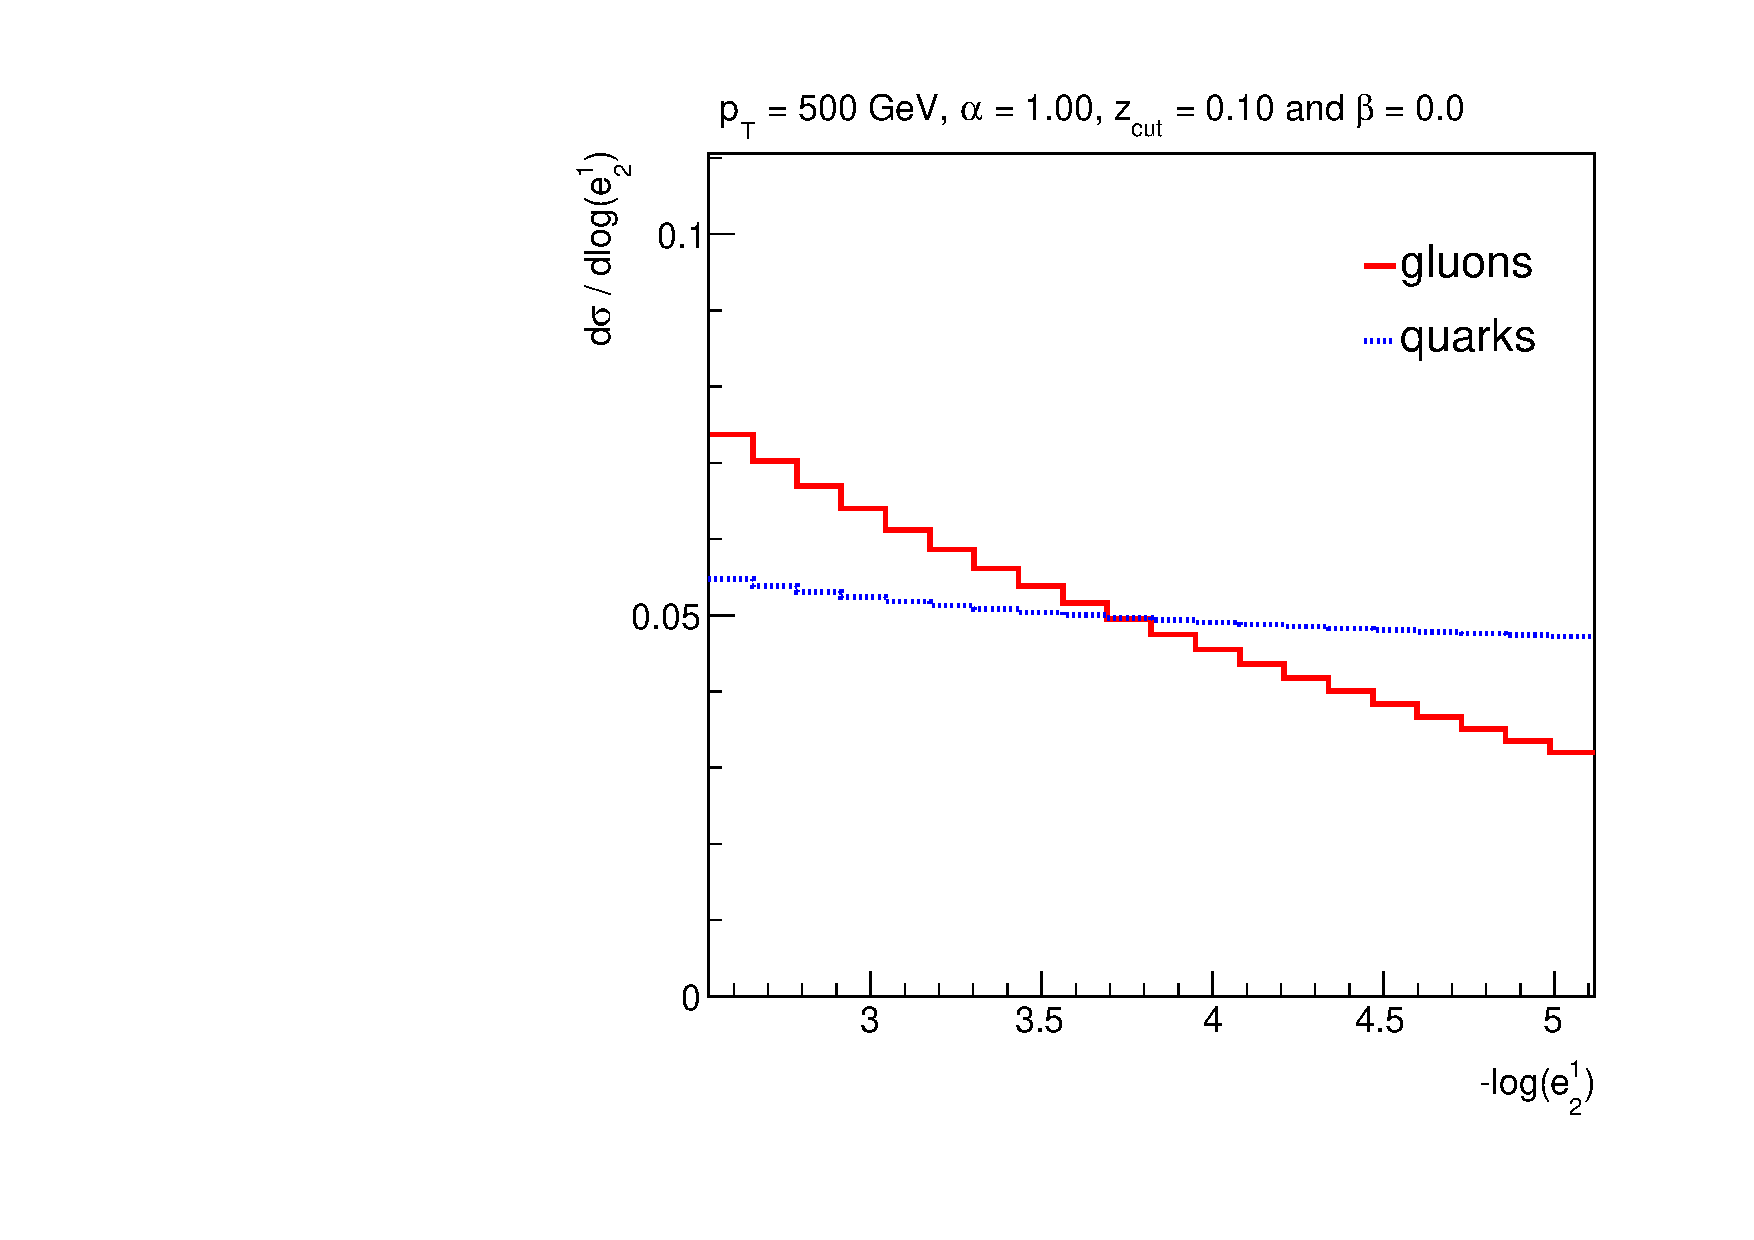
\includegraphics[width = 0.49\columnwidth]{figures/PDFs_alpha_10zcut1_beta_023451324.pdf}
\end{center}
\caption{The quark and gluon templates, computed at
  NLL~\cite{Marzani:2017mva,Marzani:2017kqd} for $\alpha=2$ (left),
  $\alpha=1$ (middle), and $\alpha=0.5$ (right).  Note that larger
  masses are on the left so that the non-perturbative regime is on the
  right and the fixed-order regime is on the left. }
\label{fig:templates}
\end{figure}
	
\begin{figure}[h!]
\begin{center}
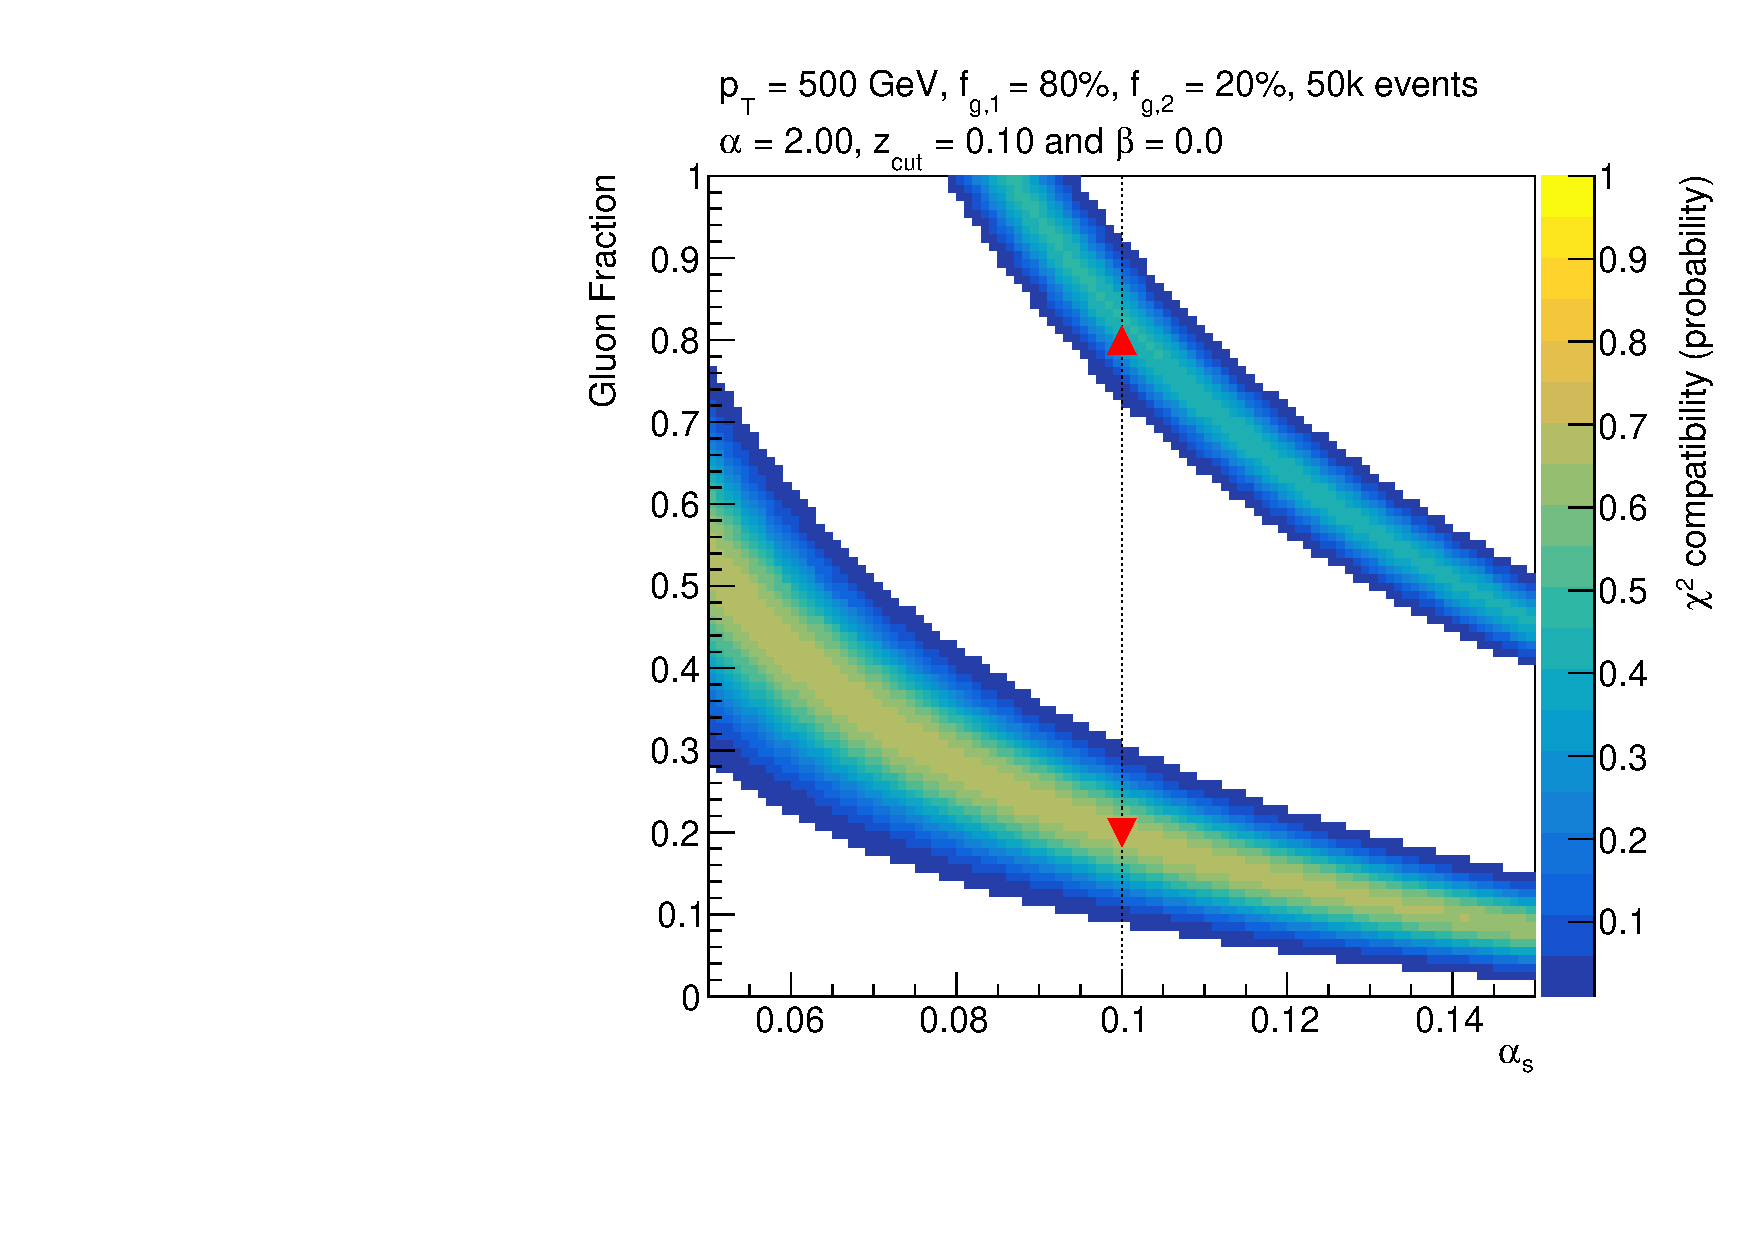
\includegraphics[width = 0.49\columnwidth]{figures/banana_alpha_20beta_0_zcut_123451324.pdf}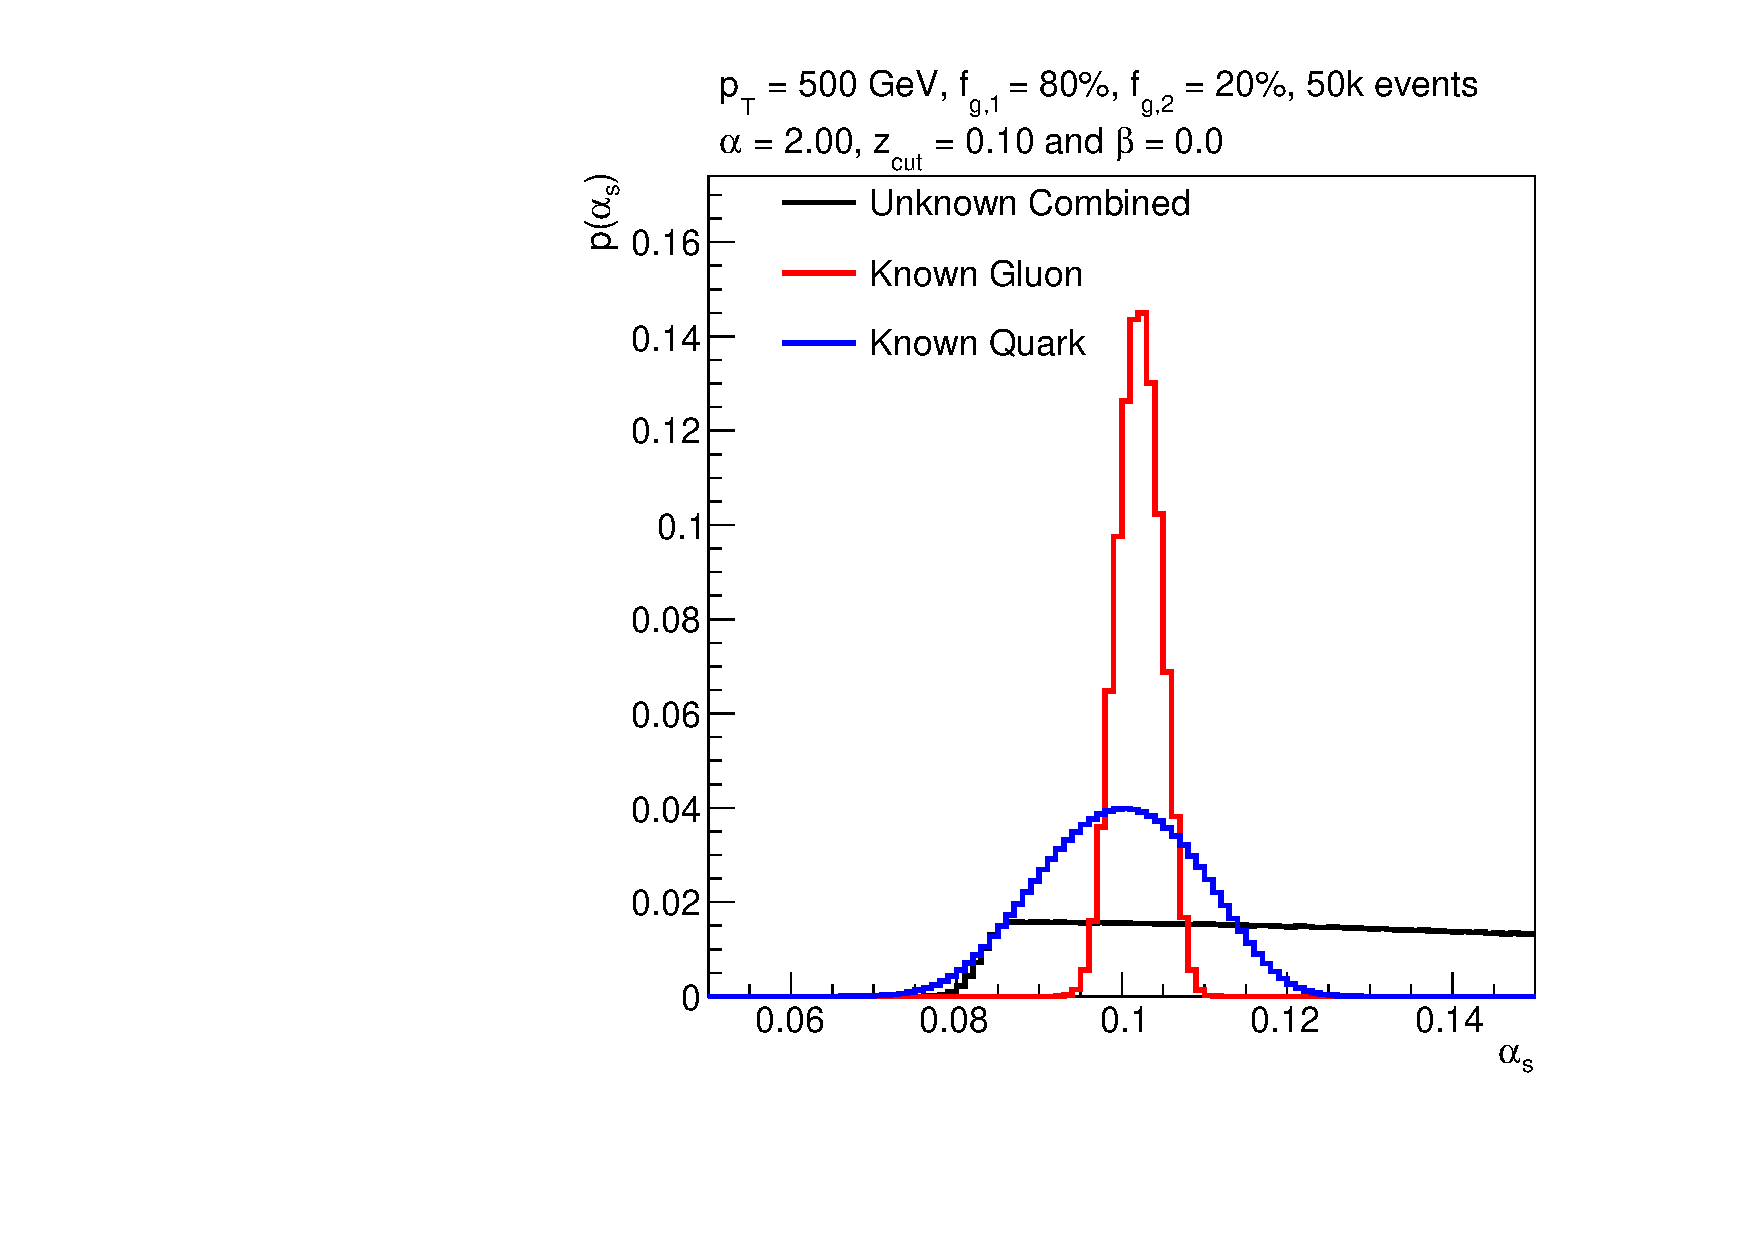
\includegraphics[width = 0.49\columnwidth]{figures/palpha_alpha_20beta_0_zcut_123451324.pdf}
\end{center}
\caption{Left: the probability of the minimized $\chi^2$ (assuming
  $n_\text{bins}-1$ degrees of freedom) from Eq.~\ref{eq:chi2fit} as a
  function of $f_g$ and $\alpha_s$ for a sample with 80\% gluons and
  one with 80\% quarks.  The true value of $\alpha_s$ is 0.1, as indicated by triangle markers.  Right: The right plot marginalized over $f_g$
  and normalized to unity.  The three lines correspond to the fit performed on a pure sample of quarks, a pure sample of gluons, or a mixed sample of ($f_g\in\{0.2,0.8\}$) where the fractions are not known a priori.  This is the result from one pseudo-experiment with 100k events.}
\label{fig:alpha2fit}
\end{figure}

%   \gs{The legend on the
%    right plot is potentially misleading, I'd say ``known $f_g=20\%$''
%    and ``known $f_g=80\%$''. If easily doable, it might also be good
%    to have the extracted alphas (central value+uncertainty).} \gs{Why
%    has the left plot changed that much compared to the previous
%    version?} 

One way to improve the situation is to combine multiple $\alpha$, $\beta$, and $z_\text{cut}$ values (only $\alpha$ and $\beta$ are varied here).  Figure~\ref{fig:morebananas} shows the $f_g,\alpha_s$ fit for the $\alpha,\beta$ values from Fig.~\ref{fig:templates} that were not shown in Fig.~\ref{fig:alpha2fit}.  As in Fig.~\ref{fig:alpha2fit}, there are two banana-shaped regions that correspond to the $f_g=20\%$ and $f_g=80\%$ samples.   The tilt of the bananas is slightly different than the $\alpha=2, \beta=0$ case and so there is a possibility to gain from combining the information in the observables.  In practice, a challenge with this extraction is the need to understand correlations between observables.  At the moment, there are no available calculations of joint distributions of angularities.  Figure~\ref{fig:combo} shows the result of a combined fit that assumes all four distributions are statistically independent.  This is a very strong assumption that is likely not even approximately true.  However, the fact that having different tilts in the $f_g,\alpha_s$ plane is clearly shown and would be a generic feature of a multi-observable fit, even if the size of the gain is not as significant. 

%\gs{Varying $z_{\text{cut}}$ and $\beta$ would also change the slope
%  (maybe not in the 2d maps), so we could add something saying that it
%  would be interesting to study those variations as well.} 

\begin{figure}[h!]
\begin{center}
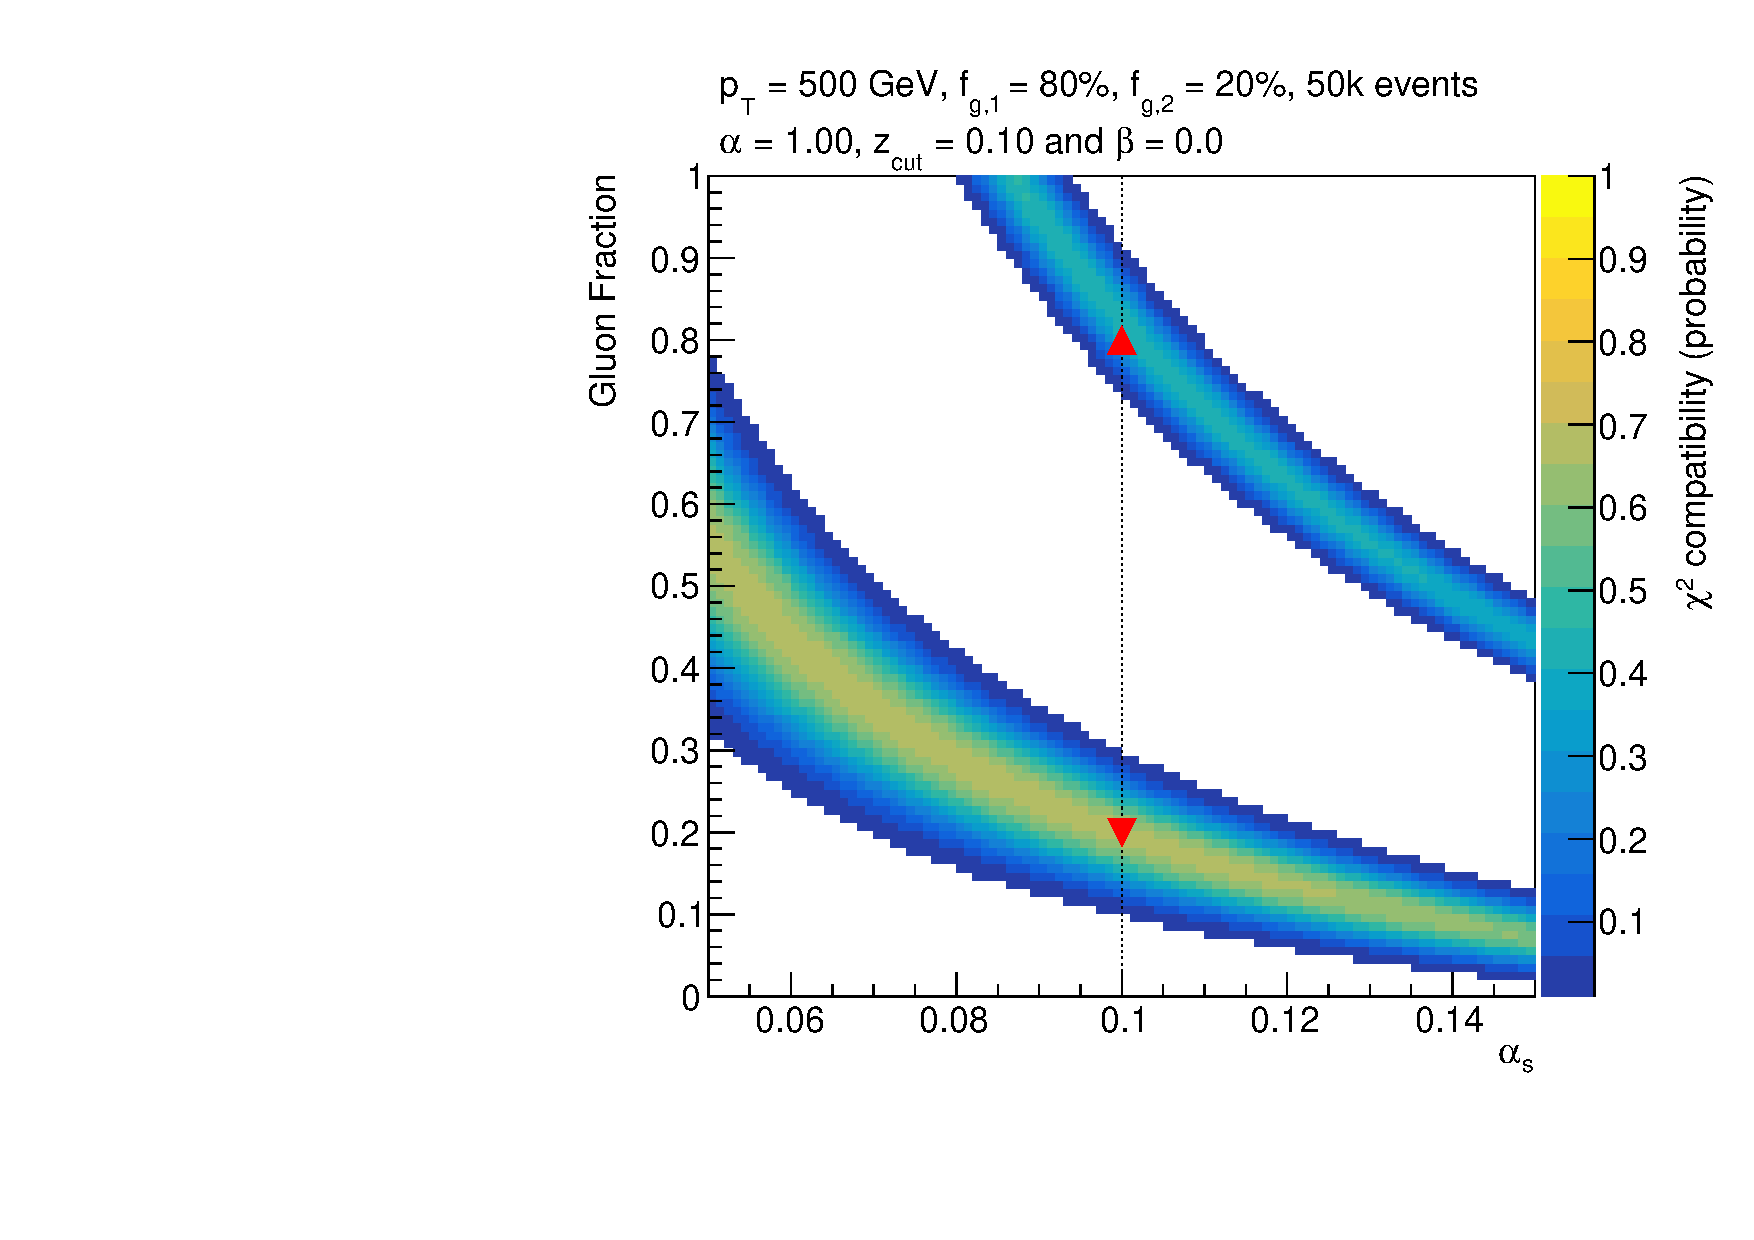
\includegraphics[width = 0.49\columnwidth]{figures/banana_alpha_10beta_0_zcut_123451324.pdf}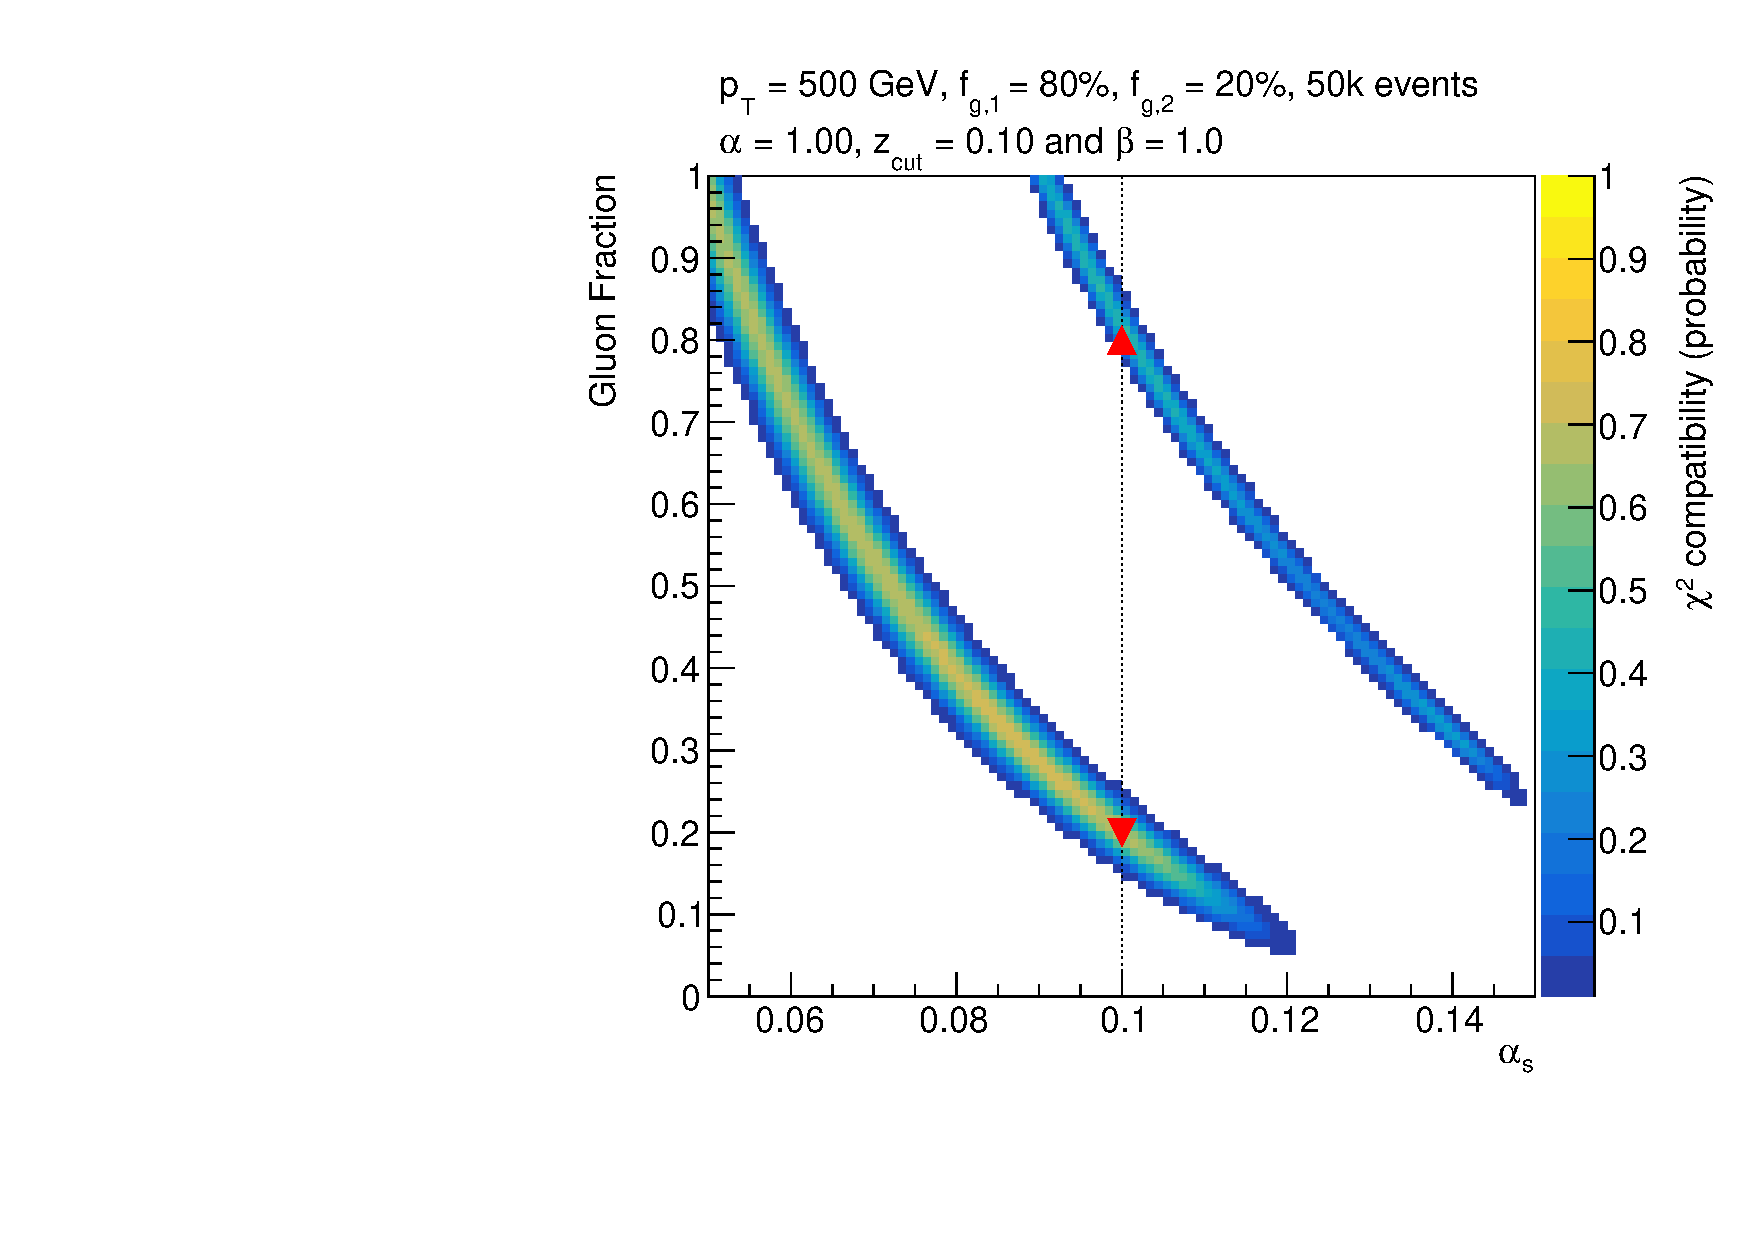
\includegraphics[width = 0.49\columnwidth]{figures/banana_alpha_10beta_10_zcut_123451324.pdf}\\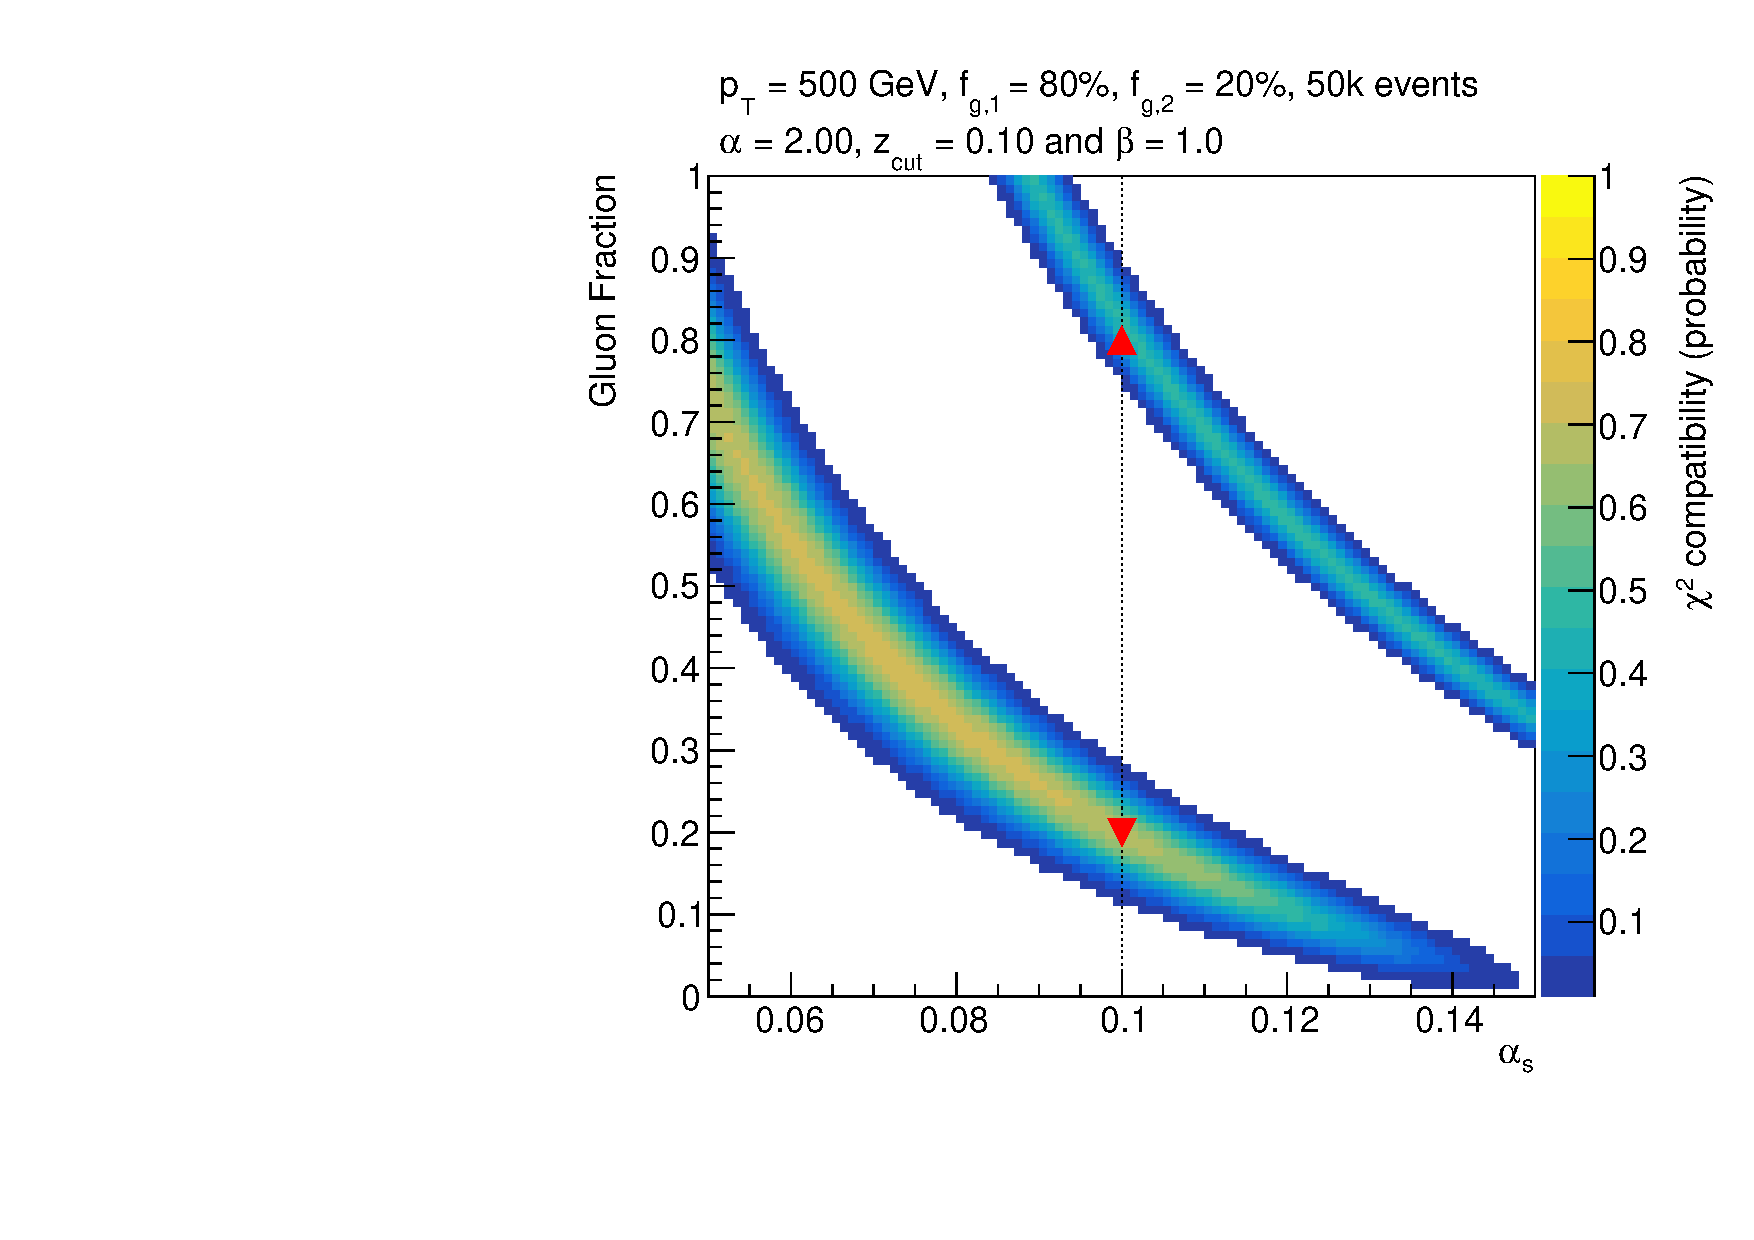
\includegraphics[width = 0.49\columnwidth]{figures/banana_alpha_20beta_10_zcut_123451324.pdf}
\end{center}
\caption{The same as the left plot of Fig.~\ref{fig:alpha2fit}, but with $\alpha=0.5$ (left) and $\alpha=1.0$ (right).}
\label{fig:morebananas}
\end{figure}

\begin{figure}[h!]
\begin{center}
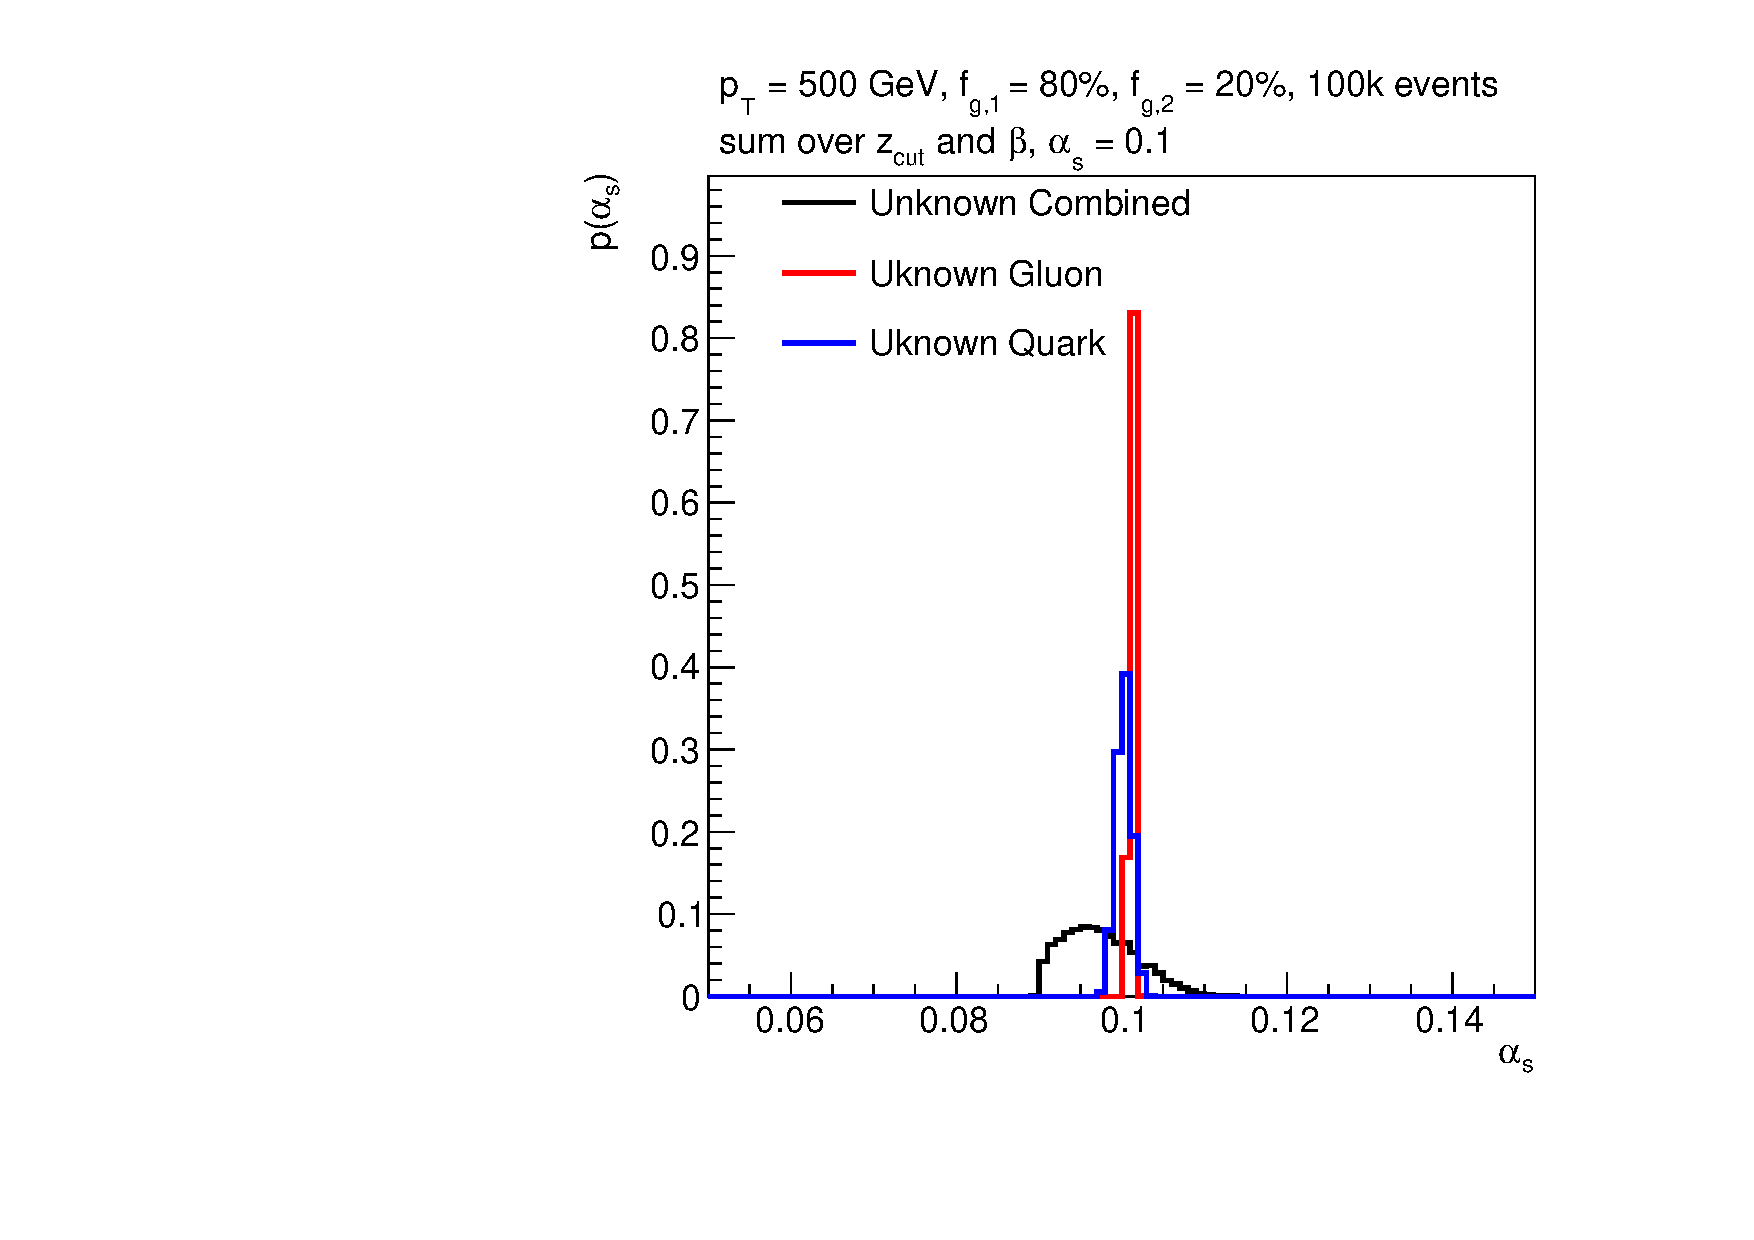
\includegraphics[width = 0.49\columnwidth]{figures/combination23451324.pdf}
%combination23451324
\end{center}
\caption{Marginalizing the $f_g,\alpha_s$ fit over the gluon fraction for a fit that combines $\alpha=0.5, 1.0$, and $2.0$.  The unknown combined mixture uses two samples with $f_g=20\%$ and $f_g=80\%$.}
\label{fig:combo}
\end{figure}

\subsection{Estimate of Experimental Resolution}
\label{sec:resolution}

To keep pace with precise theory predictions, the experimental
resolution must be well-understood in order to ensure both precision
and accuracy of the measurement.  In order to estimate the impact of
detector resolutions on the picture illustrated in
Sec.~\ref{sec:templates}, a fast simulation from Delphes
3.4.1~\cite{deFavereau:2013fsa} was studied using particle-level input
from \pythia.210. The setup uses a CMS-like detector with jets built from
particle-flow objects.  There are generically two regimes for
determining the experimental resolution.  At high mass, there are
well-resolved hard prongs in the jet and so the resolution is set by
the jet energy resolution of those `sub-jets'.  In contrast, at low
mass, the groomed jet is defined by nearly collinear splittings at
which point the angular resolution can dominate.
Figure~\ref{fig:resolution} shows the fractional $e_2^{(2)}$
resolution.  The resolution is smallest at high mass due to the excellent energy resolution of the CMS-like detector.  The
resolution at low mass is about 10\% near 15 GeV and reaches 30\% near
the limit of $\mathcal{O}(\text{few GeV})$.

\begin{figure}[h!]
\begin{center}
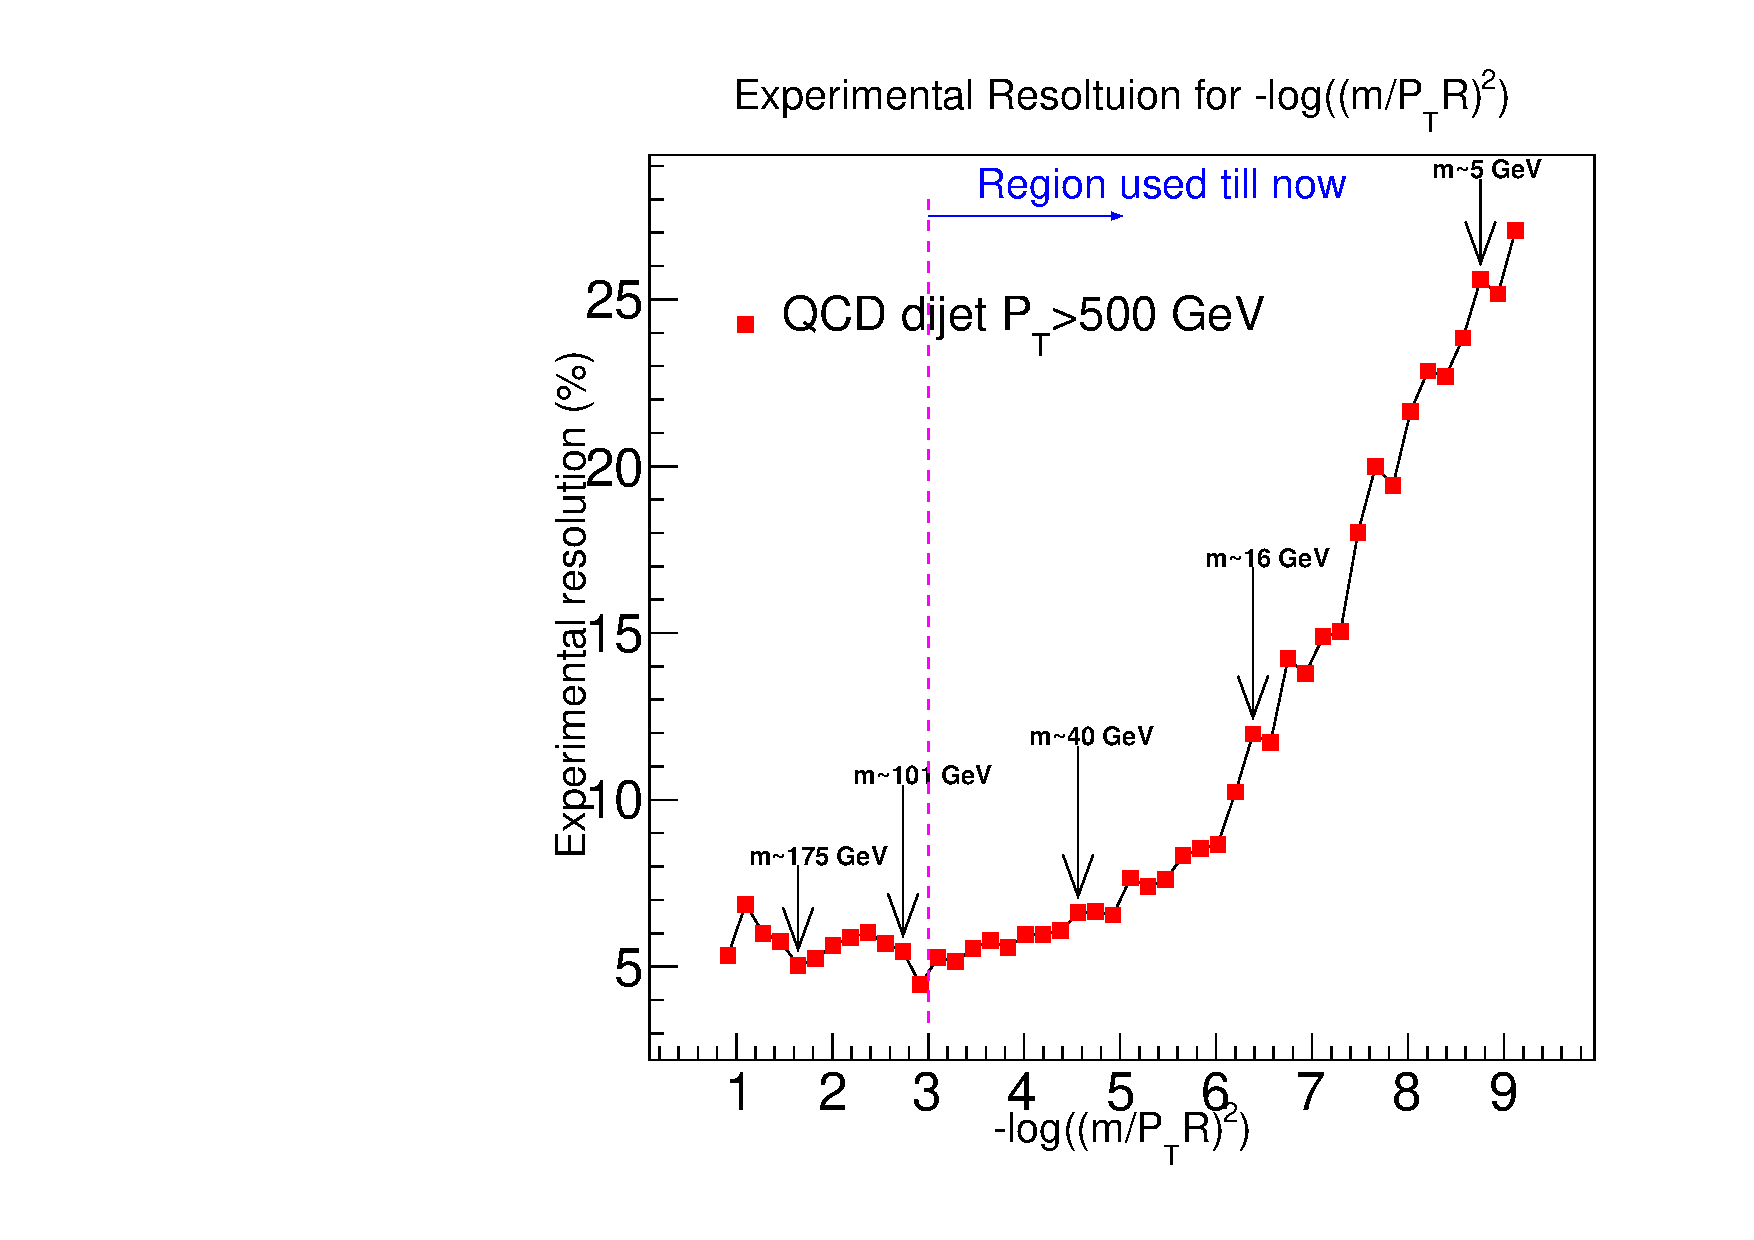
\includegraphics[width = 0.49\columnwidth]{figures/experimentaldemo/Resolution_plot_logrho_updated.pdf}
\end{center}
\caption{The fractional $e_2^{(2)}$ determined from dijet events simulated with \pythia + Delphes.  Arrows indicate the mass at given values of the angularity (add arrows for 5 or 10 GeV?).  The upper bound of the resummation regime is indicated by a dashed line.  Larger masses are to the left.}
\label{fig:resolution}
\end{figure}

As a check that the estimate resolution is sensible,
Fig.~\ref{fig:expres} compares the migration matrix between
particle-level and detector-level between Delphes and the recent ATLAS
measurement~\cite{Aaboud:2017qwh}.  The migration is qualitatively the
same, with an excellent diagonal behavior (low migrations) at high
mass and a worse resolution at low mass.  To understand the
sensitivity to jet mass scale and resolution uncertainties,
pseudo-experiments are conducted by sampling from the templates
described in Sec.~\ref{sec:templates}, smearing with the migration
matrix shown in the left plot of Fig.~\ref{fig:expres}, and then unfolding with another migration matrix that has the jet mass scale shifted or smeared by a fixed amount, and then measuring $\alpha_s$ via Eq.~\ref{eq:chi2fit} but for fixed and known $f_g=0$.  The results of this procedure are shown in Fig.~\ref{fig:expfit}.  There is little sensitivity to the jet mass resolution while there is a large uncertainty in the measured $\alpha_s$ from an uncertainty in the jet mass scale that exceeds a few percent.  Current jet mass scale uncertainties are below $5\%$ and resolution uncertainties are below 20\%~\cite{ATLAS-CONF-2017-063,CMS-PAS-JME-16-003}.  The mass scale uncertainty is as small as $2\%$ in various regions of phase space.  Therefore, it seems like a $\sim 10\%$ measurement of $\alpha_s$ is feasible, as the uncertainty on the jet mass reaches the same level of maturity as the jet energy over the next years.

\begin{figure}[h!]
\begin{center}
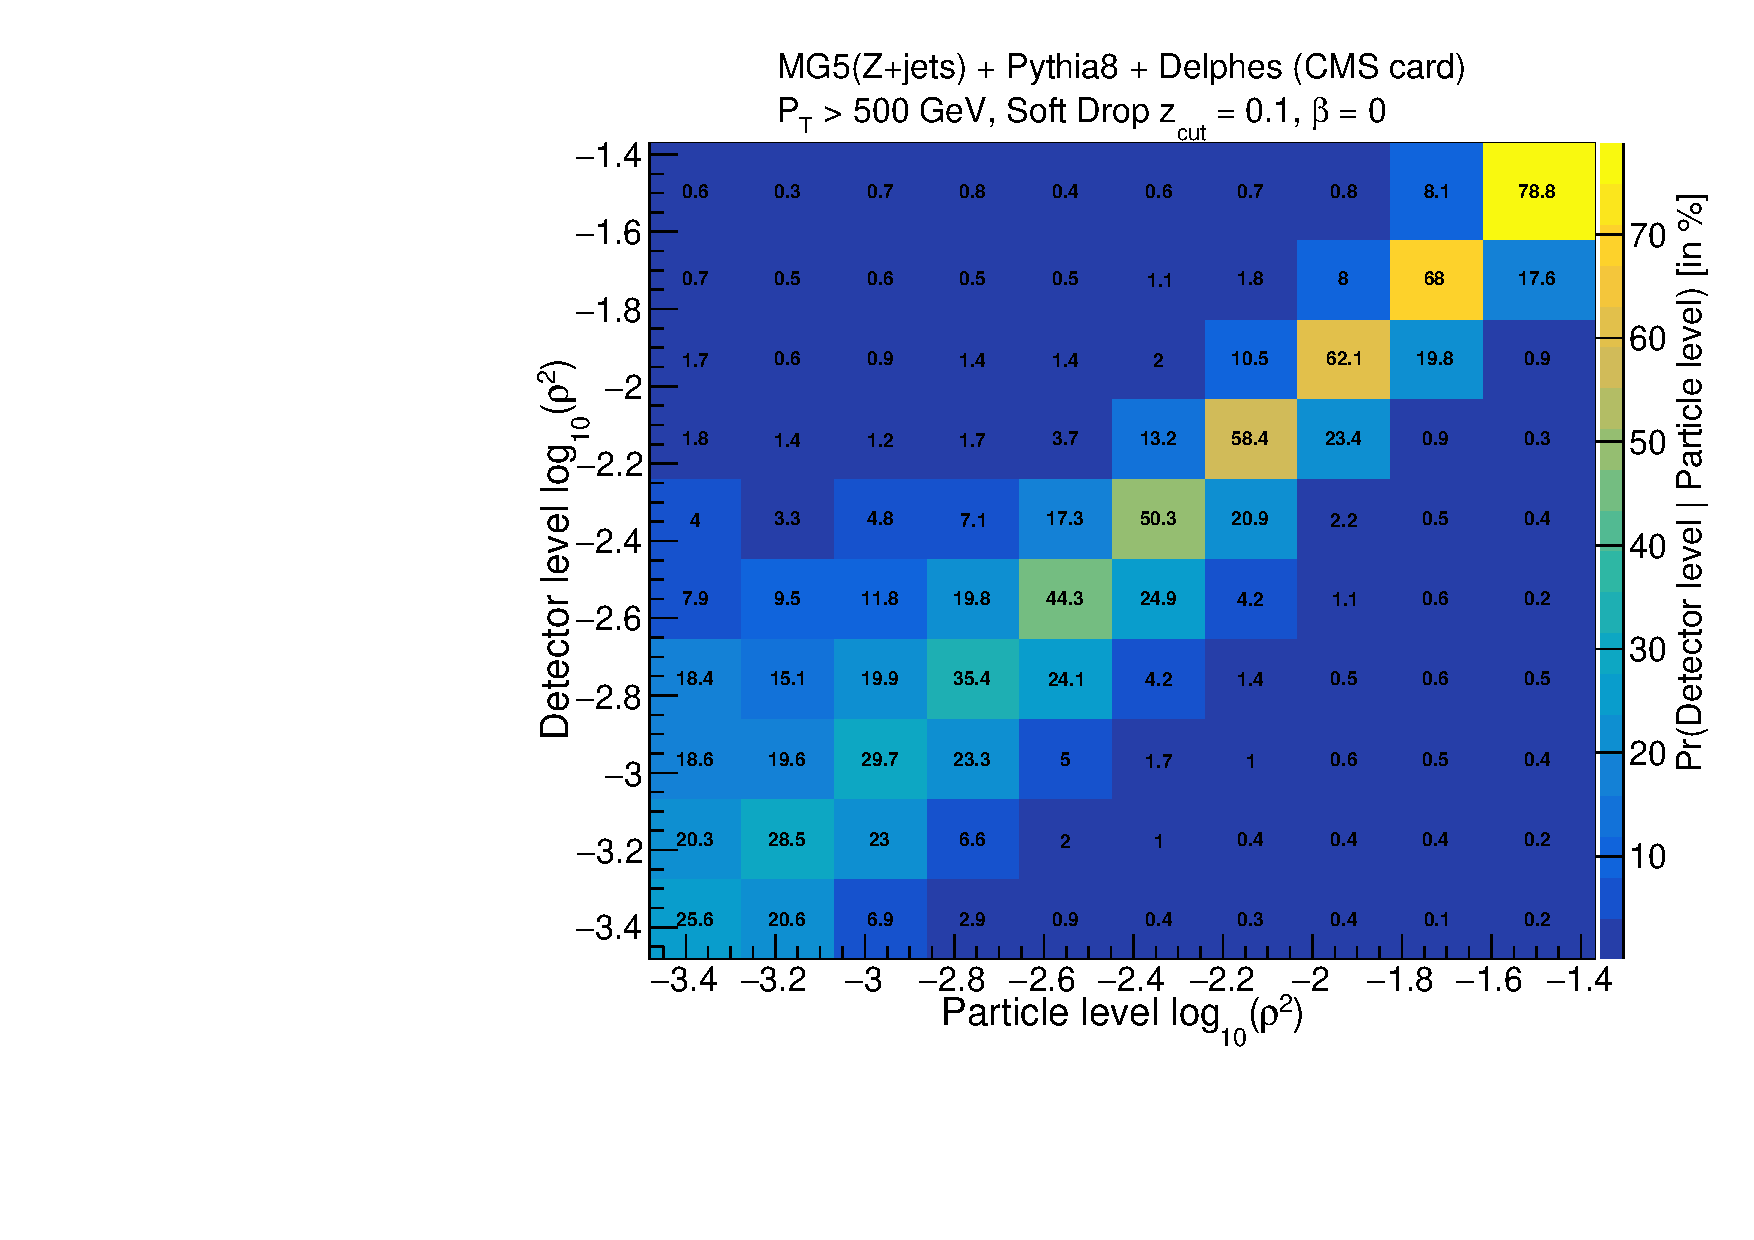
\includegraphics[width = 0.49\columnwidth]{figures/experimentaldemo/Rho_2D.pdf}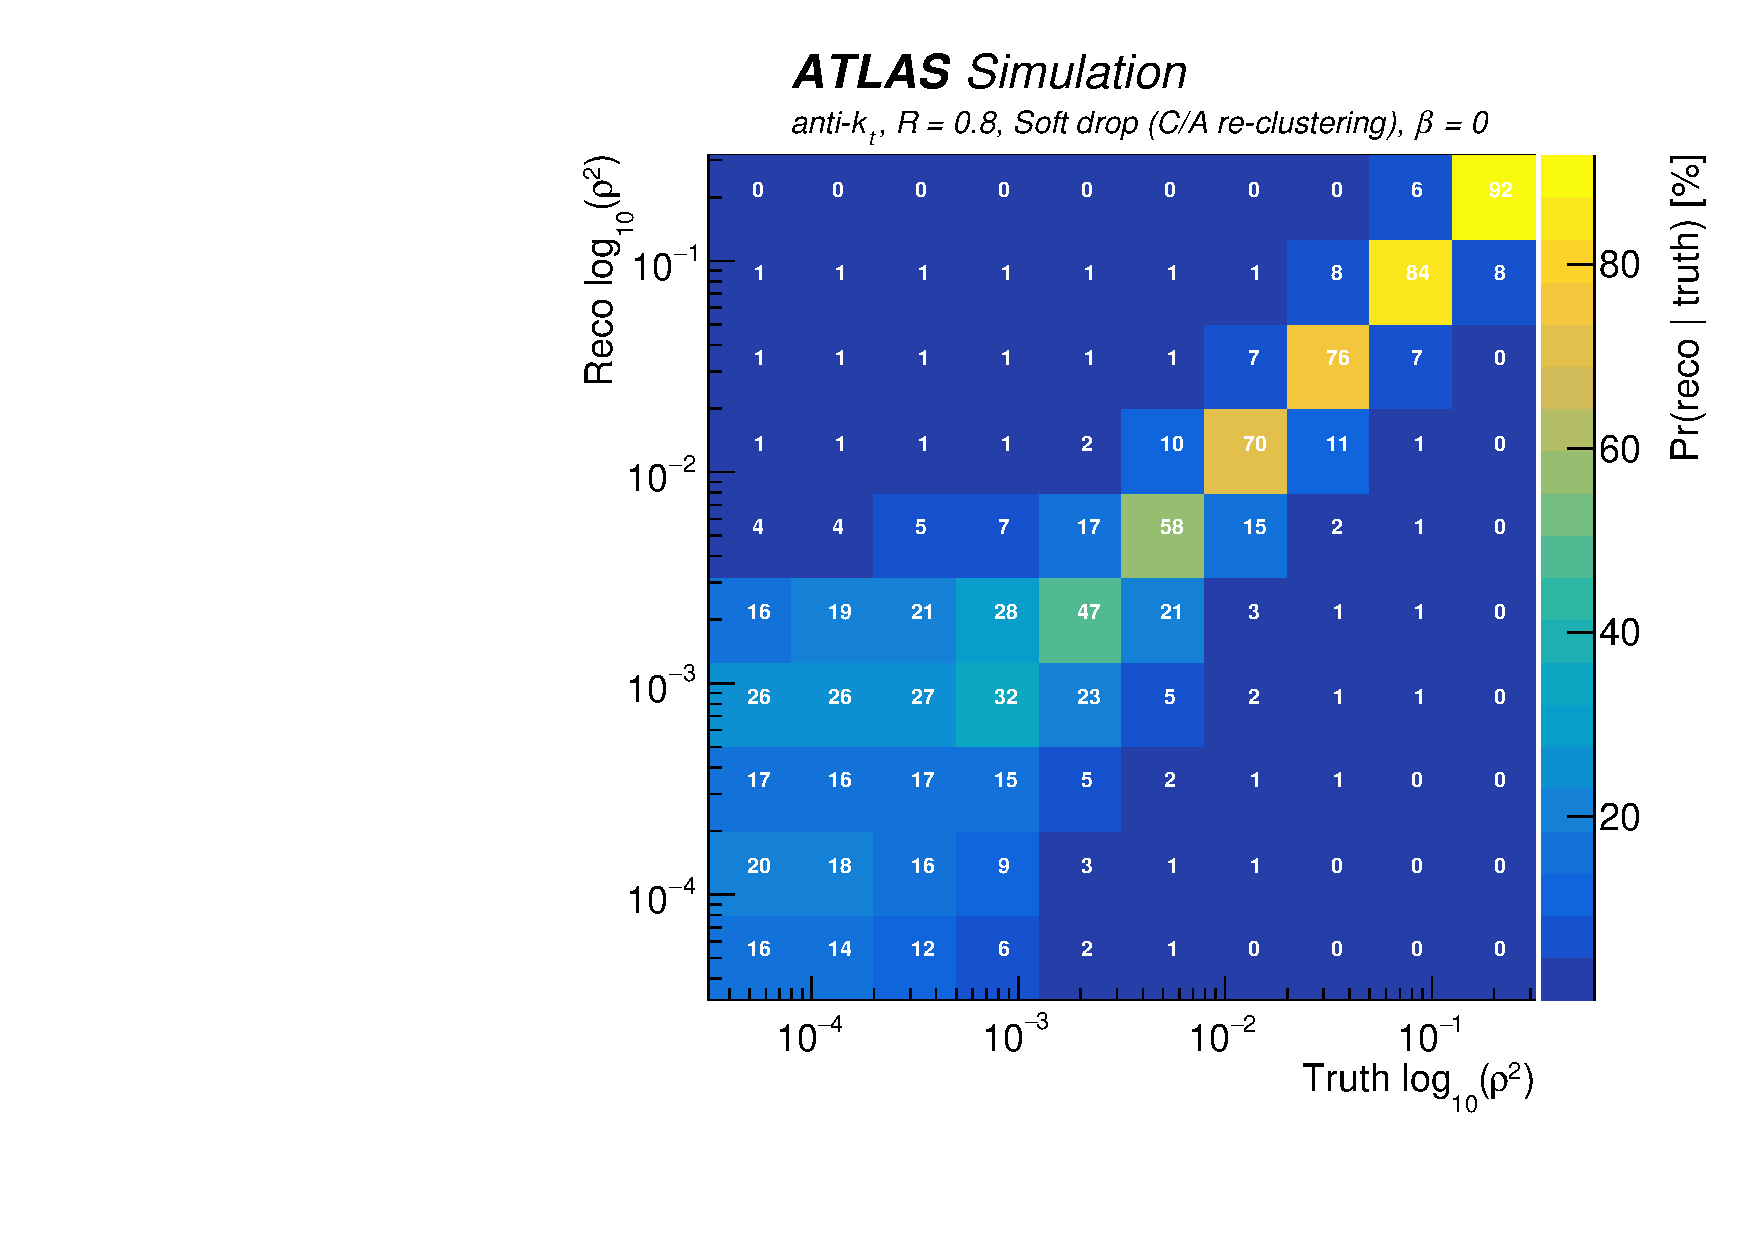
\includegraphics[width = 0.49\columnwidth]{figures/figaux_03a.pdf}
\end{center}
\caption{Left: The migration matrix between particle-level and detector-level using the Delphes simulation (left) and from the ATLAS measurement (Right; reproduced from Ref.~\cite{Aaboud:2017qwh}).  Unlike previous plots, larger masses are on the right (shown this way to match the ATLAS result). }
\label{fig:expres}
\end{figure}

\begin{figure}[h!]
\begin{center}
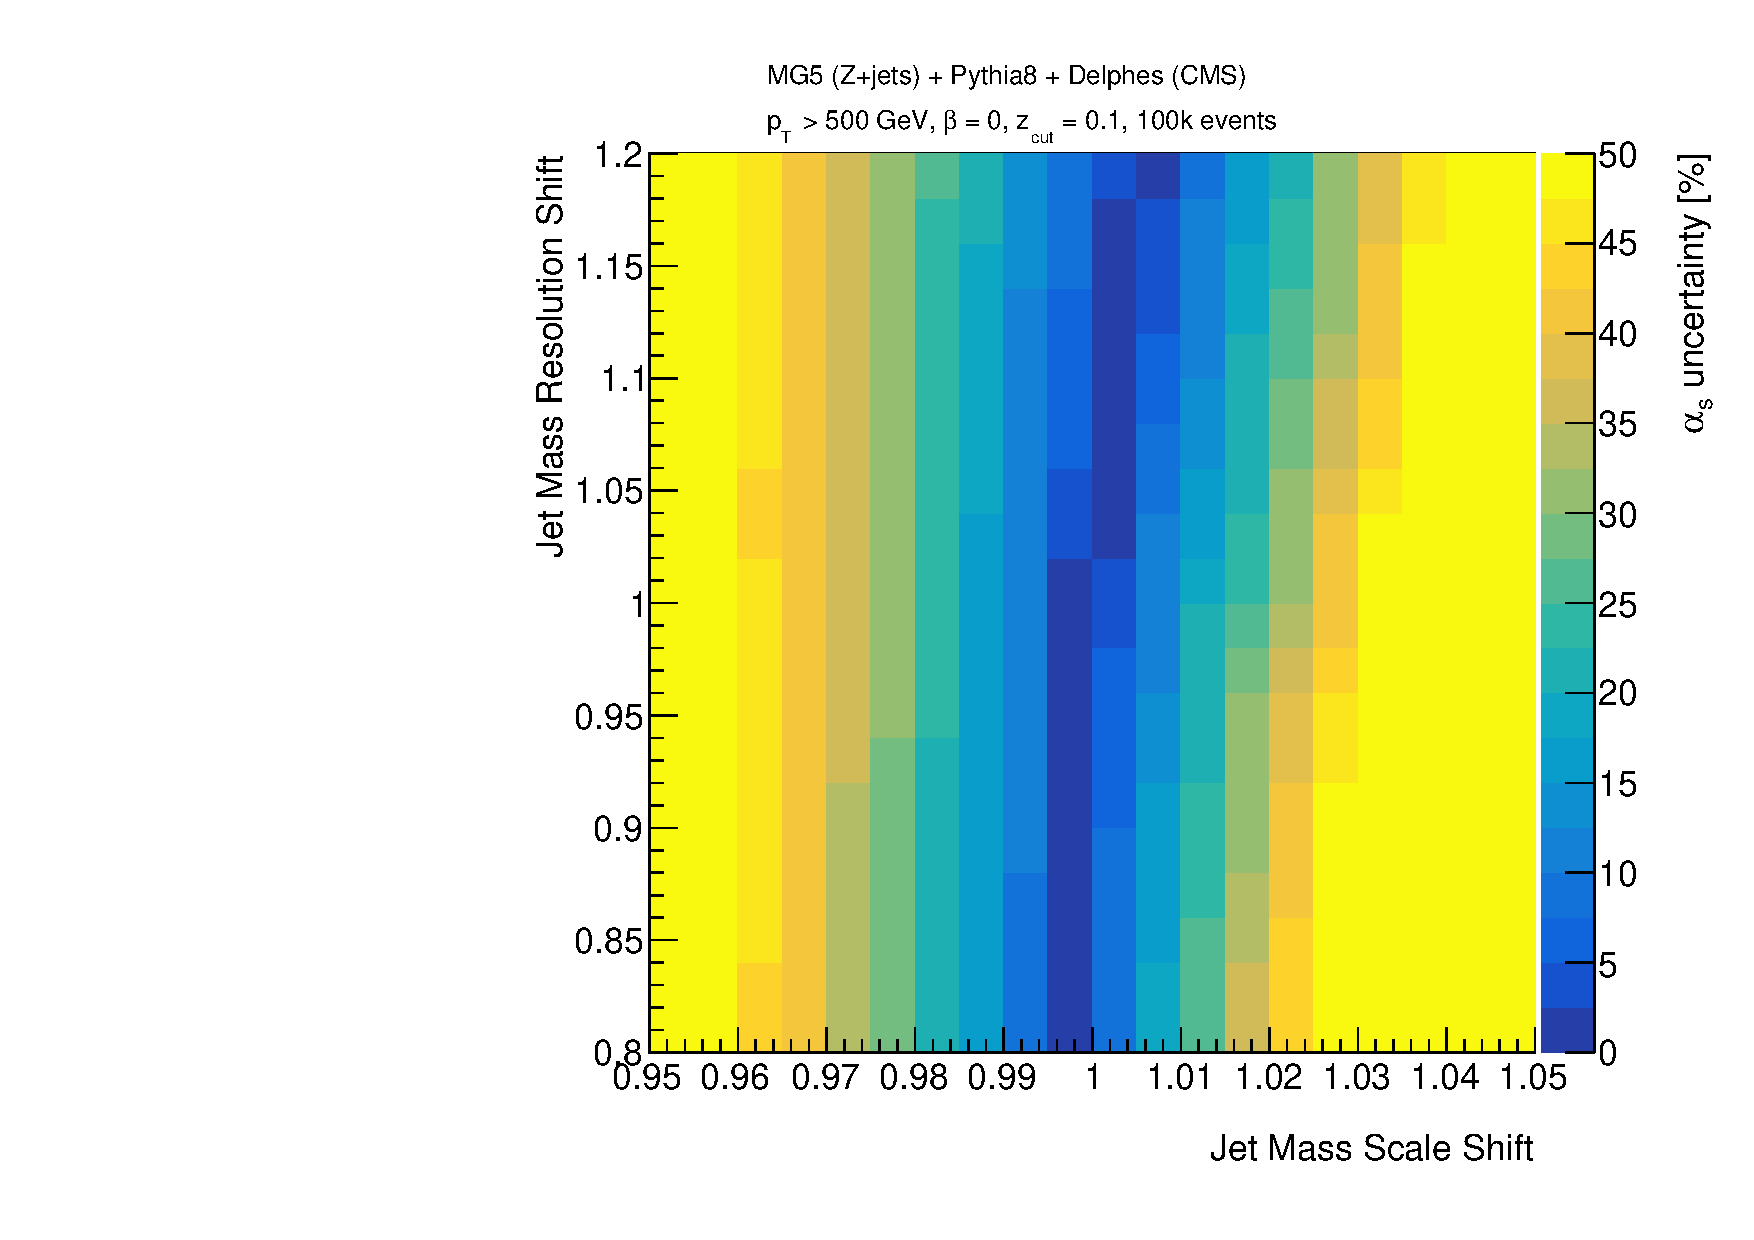
\includegraphics[width = 0.49\columnwidth]{figures/experimentaldemo/resolution_scan.pdf}
\end{center}
\caption{The impact of jet mass scale and jet mass resolution uncertainties on the uncertainty in the measured value of $\alpha_s$.  See the text for details.}
\label{fig:expfit}
\end{figure}














\begin{comment}
\subsection{Fit in Pure Quark/Gluon Samples}

Fit Methodology:
	Which fix range (minimizing theory and experimental uncertainties)?
	Constraining quark vs gluon fraction (varying SD parameters)?
	Zeroth-order feasibility study
	
	Plot is for distribution folded over PDFs (can we get rid of that?)

	Choice of jet radius (varying resummation scale)

Assume (for this section) limited by experimental uncertainties



\subsection{Constraining Quark/Gluon Fraction with Data}

	Question:  constrain quark/gluon fraction (adjust $z_cut$)?
	Need to decide beta and zcut values
	Need to matching to fixed order
	beta = 0 mass is baseline
	
	
	Another study to mitigate quark/gluon fraction uncertainties
	Sensitivitity to PDF only to the extent of getting quark/gluon fraction
	Can mitigate that with fit.
\end{comment}

